\documentclass{article}
\usepackage[a4paper,scale=0.8,hcentering,bindingoffset=8mm]{geometry} % A4纸大小,缩放80%,设置奇数页右边留空多一点
\usepackage{hyperref}      % 超链接
\usepackage{listings}      % 代码块
\usepackage{courier}       % 字体
\usepackage{fontspec}      % 字体
\usepackage{fancyhdr}      % 页眉页脚相关宏包
\usepackage{lastpage}      % 引用最后一页
\usepackage{amsmath,amsthm,amsfonts,amssymb,bm} %数学
\usepackage{graphicx}      % 图片
\usepackage{subcaption}    % 图片描述
\usepackage{longtable,booktabs} % 表格
\usepackage{ctex}
\usepackage{soul}
\usepackage{dot2texi}
\usepackage{tikz}
\usepackage{multirow}
\usepackage{float}
% \setmainfont{Noto Sans Kaithi}
\usetikzlibrary{automata, positioning, arrows}
\lstset{                  %设置代码块
         basicstyle=\footnotesize\ttfamily,% 基本风格
         numbers=left,    % 行号
         numbersep=10pt,  % 行号间隔 
         tabsize=4,       % 缩进
         extendedchars=true, % 扩展符号?
         breaklines=true, % 自动换行
         language=C,
         frame=leftline,  % 框架左边竖线
         xleftmargin=5pt,% 竖线左边间距
         showspaces=false,% 空格字符加下划线
         showstringspaces=false,% 字符串中的空格加下划线
         showtabs=false,  % 字符串中的tab加下划线
 }
\pagestyle{fancy}         % 页眉页脚风格
\fancyhf{}                % 清空当前设置
\fancyfoot[C]{\thepage\ / \pageref{LastPage}}%页脚中间显示 当前页 / 总页数,把\label{LastPage}放在最后
\begin{document} 
    \begin{titlepage}       % 封面
        \centering
        
\includegraphics[width=\textwidth]{../SUSTC_LOGO.png}
        % \vspace*{\baselineskip}
        \rule{\textwidth}{1.6pt}\vspace*{-\baselineskip}\vspace*{2pt}
        \rule{\textwidth}{0.4pt}\\[\baselineskip]
        {\LARGE COMPILIER @Liu Yepang 2019\\[\baselineskip]\small for SUSTech CSE}
        \\[0.2\baselineskip]
        \rule{\textwidth}{0.4pt}\vspace*{-\baselineskip}\vspace{3.2pt}
        \rule{\textwidth}{1.6pt}\\[\baselineskip]
        \scshape
        \vspace*{\baselineskip}
        {\Large HomeWork 4\par }
        Edited by \\[\baselineskip] {汪至圆\par}
        {\Large 11610634\par }
        \vfill
        {\scshape 2019} \\{\large SHENZHEN}\par
    \end{titlepage}
    \section{Exercise 1 (Top-Down Parsing): }
    Consider the following grammar G:
    $$
        \begin{array}{c}{S \rightarrow a B} \\ {B \rightarrow S+B | \epsilon}\end{array}
    $$
        \subsection{Construct the predictive parsing table for G. [20 points]}
            $$
                \begin{array}{c}
                    {FIRST(S):\{a\}}\\
                    {FIRST(B):\{a,\epsilon\}}\\
                    {FELLOW(S)\{+,\$\}}\\
                    {FELLOW(B)\{+,\$\}}
                \end{array}
            $$
            \begin{table}[!htbp]
                \centering
                \caption{Parsing Table}
                \label{tab:aStrangeTable}
                \begin{tabular}{|c|c|c|c|}
                    \hline
                    \multirow{2}*{Non-Terminal} & \multicolumn{3}{c|}{INPUT SYMBOL}\\
                    \cline{2-4}
                    ~ & a & + & \$\\
                    \hline
                    S & $S \rightarrow a B$ & & \\
                    B & $B \rightarrow S+B$ & $B \rightarrow \epsilon$ & $B \rightarrow \epsilon$ \\
                    \hline
                \end{tabular}
            \end{table}
        \subsection{Is the grammar LL(1)? [10 points]}
            For the $B \rightarrow S+B | \epsilon$
            \begin{itemize}
                \item ${FIRST(S+B)=\{a\}}$ and ${FIRST(\epsilon)=\{\epsilon\}}$, $FIRST(S+B)\bigcup FIRST(\epsilon)=\emptyset$
                \item ${FIRST(\epsilon)=\{\epsilon\}}$, and $FIRST(S+B)\bigcup FELLOW(B)=\emptyset$
            \end{itemize}
            So $B \rightarrow S+B | \epsilon$ is LL(1)
        \subsection{Can an LL(1) parser accept the input string aaaa+++? If yes, please list the moves made by the parser; otherwise, state the reason. Before parsing, please resolve conflicts in the parsing table if any. [20 points]}
        Yes, it can
        \begin{table}[H]
            \centering
            \caption{}
            \label{tab:aStrangeTable}
            \begin{tabular}{|c|c|c|c|}
                \hline
                    Matched & Stack     & Input     & Output Action                 \\
                    \hline
                            & S\$         & aaaa+++\$   &                               \\
                    \hline
                            & aB\$        & aaaa+++\$   & Output $s\rightarrow aB$      \\
                    \hline
                    a       & B\$         & aaa+++\$    & Match a                       \\
                    \hline
                    a       & S+B\$       & aaa+++\$    & Output $B\rightarrow S+B$     \\
                    \hline
                    a       & aB+B\$      & aaa+++\$    & Output $s\rightarrow aB$      \\
                    \hline
                    aa      & B+B\$       & aa+++\$     & Match a                       \\
                    \hline
                    aa      & S+B+B\$     & aa+++\$     & Output $B\rightarrow S+B$     \\
                    \hline
                    aa      & aB+B+B\$    & aa+++\$     & Output $s\rightarrow aB$      \\
                    \hline
                    aaa     & B+B+B\$     & a+++\$      & Match a                       \\
                    \hline
                    aaa     & S+B+B+B\$   & a+++\$      & Output $B\rightarrow S+B$     \\
                    \hline
                    aaa     & aB+B+B+B\$  & a+++\$      & Output $s\rightarrow aB$      \\
                    \hline
                    aaaa    & B+B+B+B\$   & +++\$       & Match a                       \\
                    \hline
                    aaaa    & +B+B+B\$    & +++\$       & Output $B\rightarrow\epsilon$ \\
                    \hline
                    aaaa+   & B+B+B\$     & ++\$        & Match +                       \\
                    \hline
                    aaaa+   & +B+B\$      & ++\$        & Output $B\rightarrow\epsilon$ \\
                    \hline
                    aaaa++  & B+B\$       & +\$         & Match +                       \\
                    \hline
                    aaaa++  & +B\$        & +\$         & Output $B\rightarrow\epsilon$ \\
                    \hline
                    aaaa+++ & B\$         & \$          & Match +                       \\
                    \hline
                    aaaa+++ & \$          & \$          & Output $B\rightarrow\epsilon$ \\
                    \hline
            \end{tabular}
        \end{table}
    \section{Exercise 2 (Bottom-Up Parsing): Consider the grammar G in the required Exercise 1:}
        \subsection{Construct the SLR(1) parsing table for G. [20 points]}
        $\text{The CLOSURE of item set }\{[S'\rightarrow->\cdot S]\}\text{ is }
        I_0 =CLOSURE([S'\rightarrow\cdot S) = \{[S'\rightarrow\cdot S],[S\rightarrow\cdot aB]\}$
        
        So, there are:

        $I_1 = GOTO(I_0,S) = \{[S'\rightarrow S\cdot]\}$

        $I_2 = GOTO(I_0,a) = \{[S->a\cdot B],[B\rightarrow \cdot S+B],[B\rightarrow \cdot \epsilon], [S\rightarrow \cdot aB]\}$

        $GOTO(I_2,a)=I_2$

        $I_3 = GOTO(I_2, B) = \{[S\rightarrow aB\cdot]\}$

        $I_4 = GOTO(I_2,S) = \{[B\rightarrow S\cdot+B]\}$

        $I_5 = GOTO(I_4,+) = \{[B\rightarrow S+\cdot B],[B\rightarrow\cdot S+B],[B\rightarrow\cdot\epsilon],[S\rightarrow \cdot aB]\}$
        
        $GOTO(I_5,a)=I_2$

        $GOTO(I_5,S)=I_4$

        $I_6=GOTO(I_5,B)=\{[B\rightarrow S+B\cdot]\}$

        \begin{figure}[H]
            \centering
            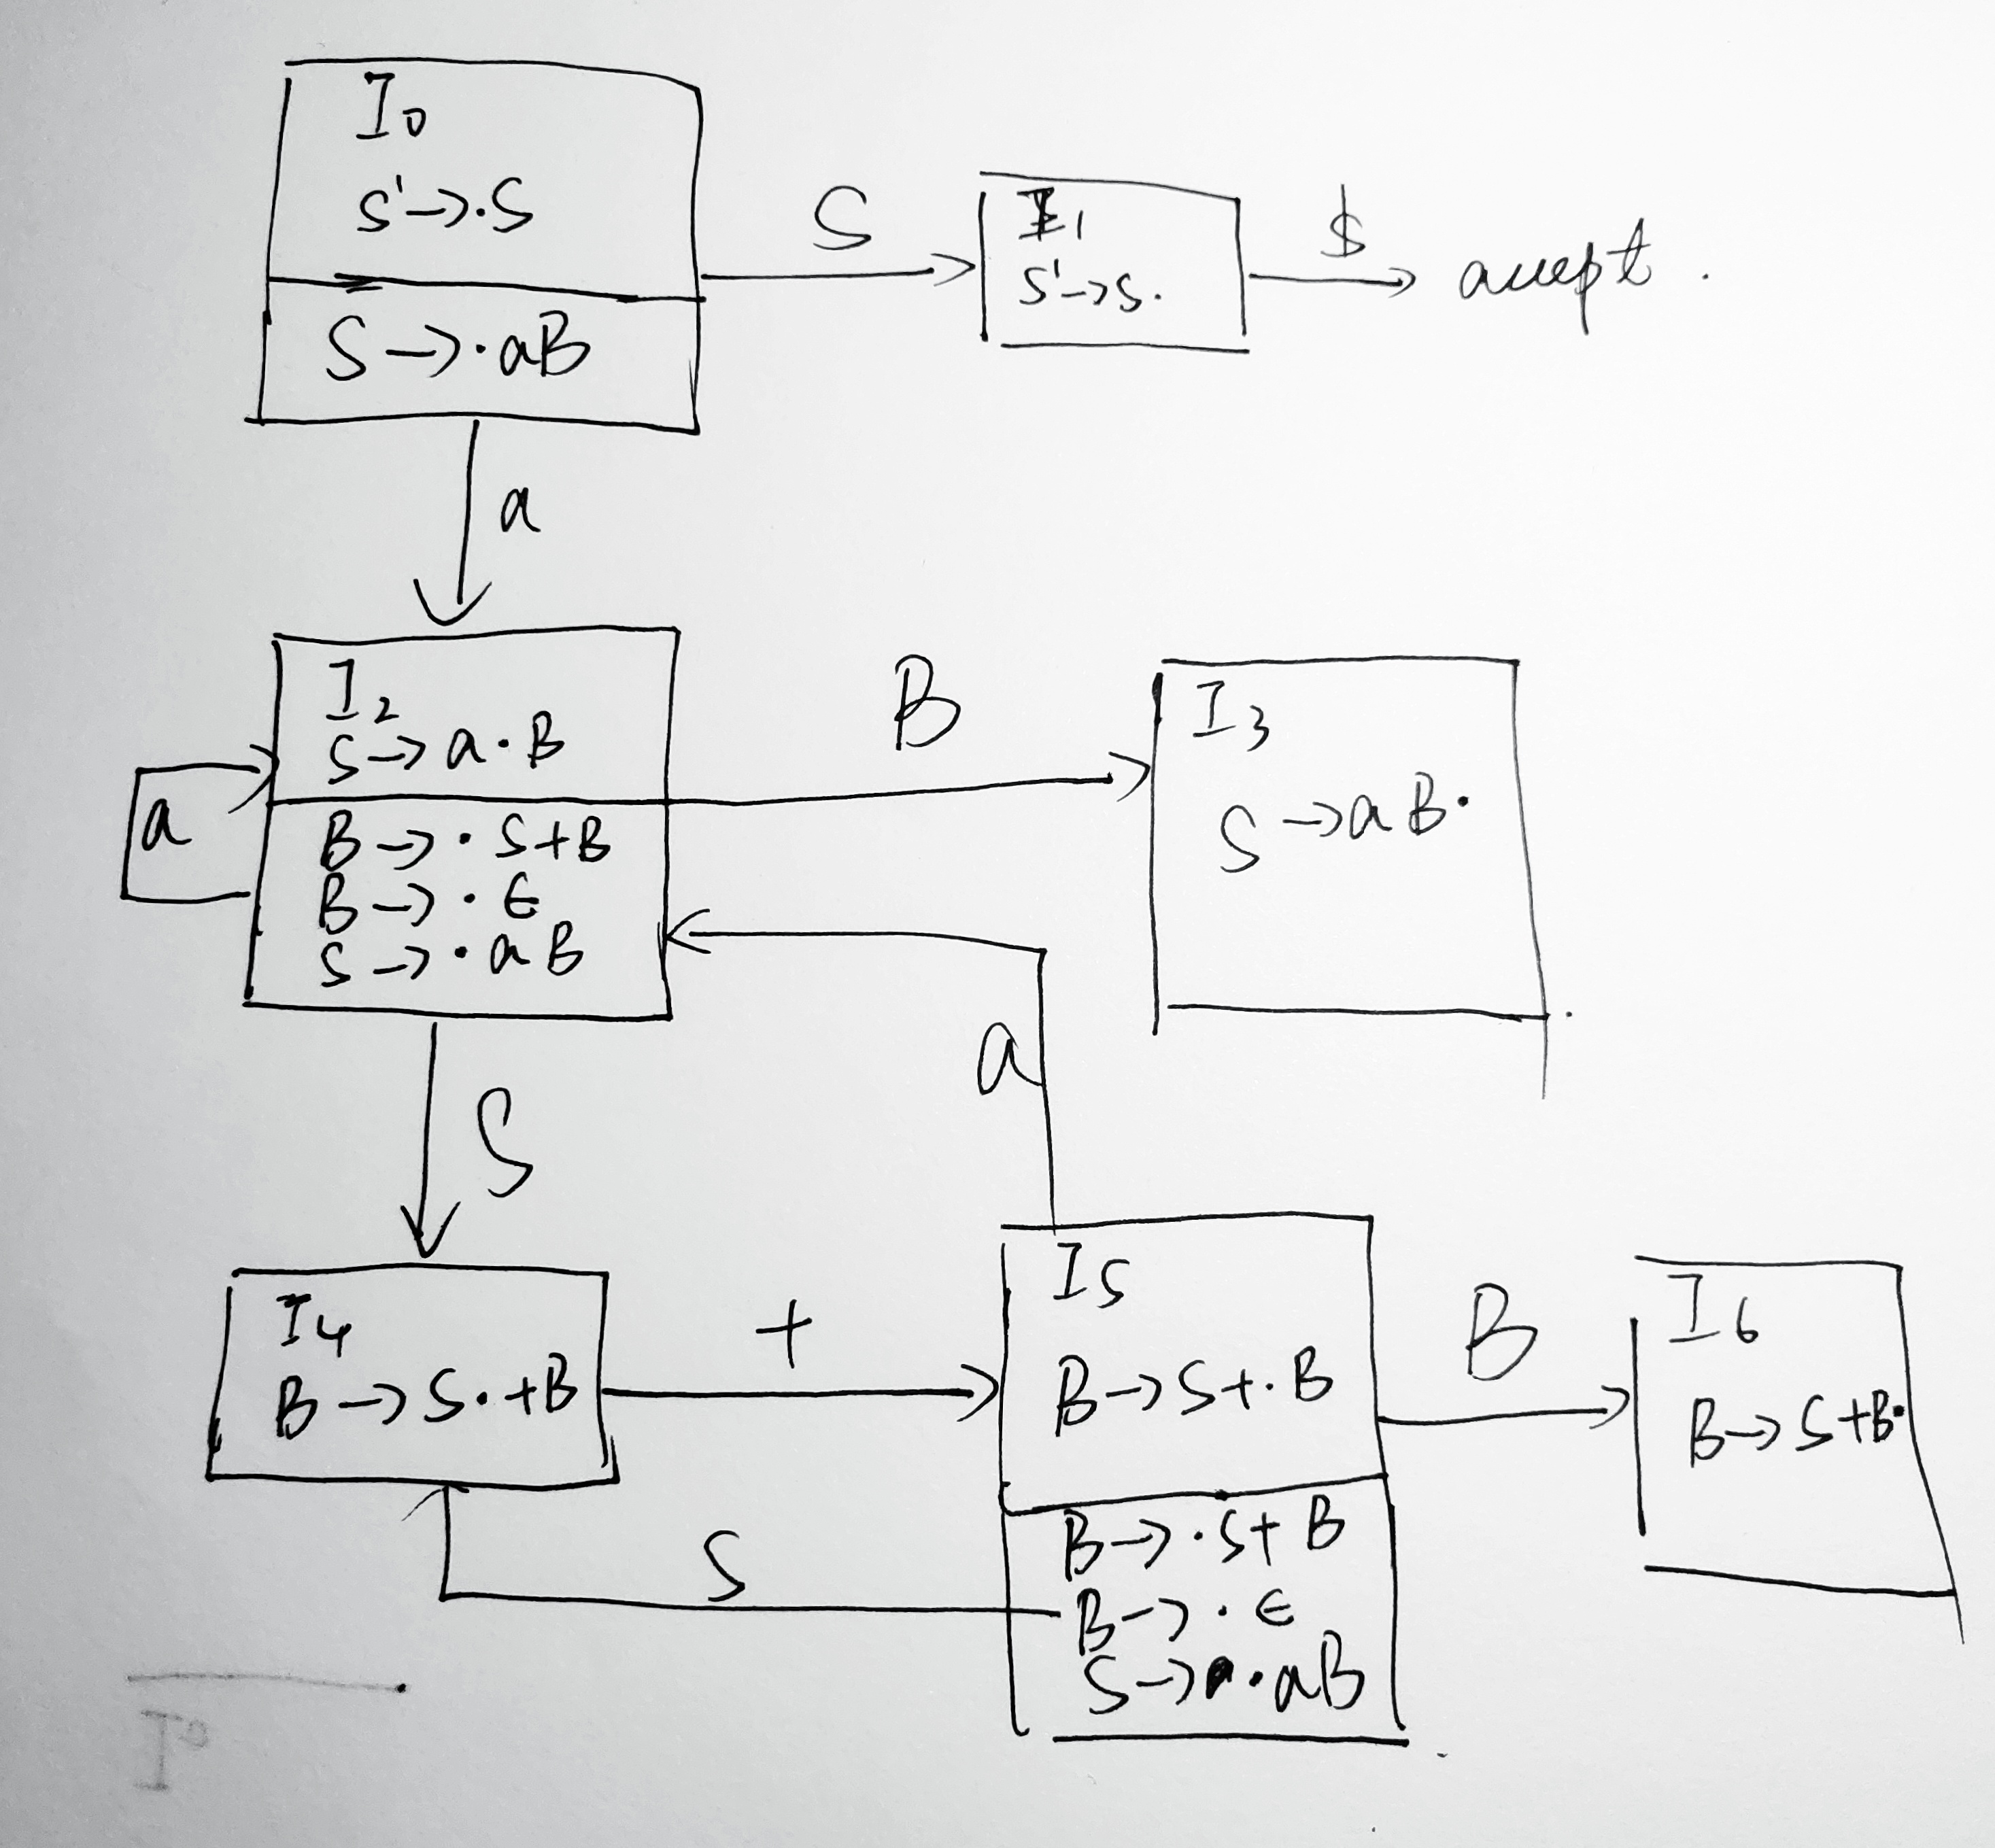
\includegraphics[scale=0.15]{./assg_4_2-1.jpg}
            \caption{}
            \label{fig:label}
            \end{figure}
        $$
            (1) S\rightarrow aB\\
            (2) B\rightarrow S+B\\
            (3) B\rightarrow \epsilon\\
        $$
        \begin{table}[H]
            \centering
            \caption{Parsing Table}
            \begin{tabular}{|c|c|c|c|c|c|}
                \hline
                \multirow{2}*{STATE} & \multicolumn{3}{c|}{ACTION} & \multicolumn{2}{c|}{GOTO} \\
                \cline{2-6}
                ~ & a & + & \$ & S & B \\
                \hline
                0 &$s_2$ & & & 1 & \\
                \hline
                1 &  & & $accept$ & & \\
                \hline
                2 & $s_2$ & $r_3$ & $r_3$ & 4 & 3 \\
                \hline
                3 & & $r_1$ & $r_1$ & & \\
                \hline
                4 & & $s_5$ & & & \\
                \hline
                5 & $s_2$ & $r_3$ & $r_3$ & 4 & 6 \\
                \hline
                6 & & $r_2$ & $r_2$ & & \\
                \hline
            \end{tabular}
        \end{table}
        \subsection{Is the grammar SLR(1)? [10 points]}
            Yes, it is, there is no conflict during the parsing table construction
        \subsection{Can an SLR(1) parser accept the input string aaaa+++? If yes, please list the moves
        made by the parser; otherwise, state the reason. Before parsing, please resolve conflicts
        if any. [20 points]}
        Yes, it can.
        \begin{table}[H]
            \centering
            \caption{}
            \begin{tabular}{|c|c|c|c|c|}
                \hline
                    & STACK     & SYMBOLS   & INPUT     & ACTION\\
                0   & 0         &           & aaaa+++\$ & Shift \\
                \hline
                1   & 02        & a         & aaa+++\$  & Shift \\
                \hline
                2   & 022       & aa        & aa+++\$   & Shift \\
                \hline
                3   & 0222      & aaa       & a+++\$    & Shift \\
                \hline
                4   & 02222     & aaaa      & +++\$     & Reduce $B\rightarrow\epsilon$ \\
                \hline
                5   & 022223    & aaaaB     & +++\$     & Reduce $S\rightarrow aB$\\
                \hline
                6   & 02224     & aaaS      & +++\$     & Shift \\
                \hline
                7   & 022245    & aaaS+     & ++\$      & Reduce $B\rightarrow\epsilon$\\
                \hline
                8   & 0222456   & aaaS+B    & ++\$      & Reduce $B\rightarrow S+B$ \\
                \hline
                9   & 02223     & aaaB      & ++\$      & Reduce $S\rightarrow aB$\\
                \hline
                10  & 0224      & aaS       & ++\$      & Shift \\
                \hline
                11  & 02245     & aaS+      & +\$       & Reduce $B\rightarrow\epsilon$ \\
                \hline
                12  & 022456    & aaS+B     & +\$       & Reduce $B\rightarrow S+B$ \\
                \hline
                13  & 0223      & aaB       & +\$       & Reduce $S\rightarrow aB$ \\
                \hline
                14  & 024       & aS        & +\$       & Shift \\
                \hline
                15  & 0245      & aS+       & \$        & Reduce $B\rightarrow\epsilon$ \\
                \hline
                16  & 02456     & aS+B      & \$        & Reduce $B\rightarrow S+B$ \\
                \hline
                17  & 023       & aB        & \$        & Reduce $S\rightarrow aB$ \\
                \hline
                18  & 01        & S         & \$        & Accept\\
                \hline
            \end{tabular}
        \end{table}

\end{document}